\documentclass[12pt, a4paper]{ctexart}

% 页面与排版设置
\usepackage[margin=2.54cm]{geometry}
\usepackage{amsmath, amssymb}
\usepackage{booktabs}
\usepackage{graphicx}
\usepackage{float}
\usepackage{color}
\usepackage{xcolor}
\usepackage{array} 
\usepackage[colorlinks=true, linkcolor=black, urlcolor=blue, citecolor=black]{hyperref}

% 代码高亮设置
\usepackage{listings}
\definecolor{codegreen}{rgb}{0,0.6,0}
\definecolor{codegray}{rgb}{0.5,0.5,0.5}
\definecolor{codepurple}{rgb}{0.58,0,0.82}
\definecolor{backcolour}{rgb}{0.96,0.96,0.96}

\lstdefinestyle{pystyle}{
    backgroundcolor=\color{backcolour},   
    commentstyle=\color{codegreen},
    keywordstyle=\color{magenta},
    numberstyle=\tiny\color{codegray},
    stringstyle=\color{codepurple},
    basicstyle=\ttfamily\small,
    breakatwhitespace=false,         
    breaklines=true,                 
    captionpos=b,                    
    keepspaces=true,                 
    numbers=left,                    
    numbersep=5pt,                  
    showspaces=false,                
    showstringspaces=false,
    showtabs=false,       
    tabsize=4
}
\lstset{style=pystyle}

\begin{document}

% ==========================================
% 自定义封面页
% ==========================================
\begin{titlepage}
\begin{center}
    ~\\[10.5pt]
    \textbf{\songti\zihao{1}  北京电影学院课程作业}
    ~\\[10.5pt] ~\\[10.5pt] ~\\[10.5pt] ~\\[10.5pt]

    {\zihao{2}\bfseries 作业1.1\\基于 PhotoResearch PR-788 光谱数据的\\显示屏白场色度学分析报告}
    
    ~\\[10.5pt] ~\\[10.5pt] ~\\[10.5pt] ~\\[10.5pt]
    ~\\[10.5pt] ~\\[10.5pt] ~\\[10.5pt] ~\\[10.5pt]
    ~\\[10.5pt] 
    
    \begin{tabular}{>{\heiti\fontsize{16pt}{16pt}\selectfont}r>{\kaishu\fontsize{16pt}{16pt}\bfseries\selectfont}l}
        作　　者：    &   祝庆\\[4pt]
        院　　系：    &   智能影像工程学院\\[4pt]
        专　　业：    &   影视技术\\[4pt]
        教学层次：    &   本科生\\[4pt]
        年　　级：    &   2023 级\\[4pt]
        学　　号：    &   231112014\\[4pt]
        指导教师：    &   顾晓娟 \hspace{0.5em} 鲁梦河\\[4pt]
        成　　绩：    &   \\[4pt]
        日　　期：    &   2026 年 3 月\\[4pt]
    \end{tabular}

\end{center}
\end{titlepage}

% 封面后重新设置页码，并生成摘要等内容
\setcounter{page}{1}

\begin{abstract}
本报告基于 PhotoResearch PR-788 测量的显示屏白场原始光谱功率分布数据（380nm - 780nm），依据 CIE 1931 标准色度观察者模型，计算了目标光源的三刺激值。报告详细探讨了常数 $k$ 在不同影像工业标准下的三种取值意义。在此基础上，推导了色品坐标（CIE 1931 $xy$ 及 CIE 1976 $u'v'$），并利用多种经典算法（McCamy、Hernández-Andrés、Robertson）交叉验证并精确计算了相关色温（CCT），为后续的监视器校准与色彩管理提供了底层数据支撑。报告中的核心色彩空间转换公式参考自 Bruce Lindbloom 的色彩学规范。
\end{abstract}

\vspace{2em}

% 生成目录
\tableofcontents

\newpage

% ==========================================
% 第一章：CIE 1931 XYZ 三刺激值计算
% ==========================================
\section{CIE 1931 XYZ 三刺激值计算}

\subsection{计算公式与理论基础}
根据 Bruce Lindbloom 提供的色彩学基础方程，由光谱功率分布 $S(\lambda)$ 计算 CIE 1931 XYZ 三刺激值的核心积分公式如下：
\begin{align}
    X &= k \int_{380}^{780} S(\lambda) \bar{x}(\lambda) \mathrm{d}\lambda \approx k \sum S(\lambda) \bar{x}(\lambda) \Delta\lambda \\
    Y &= k \int_{380}^{780} S(\lambda) \bar{y}(\lambda) \mathrm{d}\lambda \approx k \sum S(\lambda) \bar{y}(\lambda) \Delta\lambda \\
    Z &= k \int_{380}^{780} S(\lambda) \bar{z}(\lambda) \mathrm{d}\lambda \approx k \sum S(\lambda) \bar{z}(\lambda) \Delta\lambda
\end{align}

其中，$\bar{x}(\lambda), \bar{y}(\lambda), \bar{z}(\lambda)$ 为 CIE 1931 $2^\circ$ 标准观察者颜色匹配函数。由于我们在观察显示器时，视觉关注点通常集中在中央凹视场（约占据 $2^\circ$ 视角），因此采用 $2^\circ$ 匹配函数最为准确。

在色度学与影视工业色彩管理中，常数 $k$ 的取值决定了三刺激值的物理意义，通常分为三种标准化思路：
\begin{enumerate}
    \item \textbf{绝对光度学（Absolute Photometry）}：取最大光谱光视效能 $K_m = 683 \text{ lm/W}$ 作为常数 $k$。此时 $Y$ 值代表显示屏的绝对物理亮度（单位：$cd/m^2$ 或 nits），用于评估硬件发光强度。
    \item \textbf{相对色度学 - 百分比归一化（Y=100）}：取 $k = 100 / \sum S(\lambda) \bar{y}(\lambda) \Delta\lambda$。此时参考白场的 $Y$ 值恒定为 100，消除了绝对亮度差异，常用于传统色彩学计算（如 CIELAB 空间转换）及色差评估。
    \item \textbf{相对色度学 - 浮点归一化（Y=1.0）}：取 $k = 1 / \sum S(\lambda) \bar{y}(\lambda) \Delta\lambda$。此时 $Y$ 被归一化为 1.0。这是数字图像处理、CG 渲染及后期线性工作流中最常用的数据形态，便于矩阵乘法运算。
\end{enumerate}

\subsection{中间计算与最终结果}
将 PR-788 测量数据代入公式，测量步长 $\Delta\lambda = 1\text{nm}$。
首先计算基础的离散积分求和项：
\begin{align*}
    \sum S(\lambda) \bar{x}(\lambda) \Delta\lambda &\approx 1.214868 \\
    \sum S(\lambda) \bar{y}(\lambda) \Delta\lambda &\approx 1.343987 \\
    \sum S(\lambda) \bar{z}(\lambda) \Delta\lambda &\approx 1.721250
\end{align*}

代入不同的 $k$ 值，得到三种思路下的三刺激值：

\noindent\textbf{1. 绝对光度学 ($k=683$)}
\begin{itemize}
    \item $X = 683 \times 1.214868 \approx \mathbf{829.7548}$
    \item $Y = 683 \times 1.343987 \approx \mathbf{917.9431}$ （即白场亮度约为 $917.94 \text{ nits}$）
    \item $Z = 683 \times 1.721250 \approx \mathbf{1175.6139}$
\end{itemize}

\noindent\textbf{2. 相对色度学 ($Y=100$)} 
此处 $k = 100 / 1.343987 \approx 74.4055$
\begin{itemize}
    \item $X \approx \mathbf{90.3928}$
    \item $Y = \mathbf{100.0000}$ 
    \item $Z \approx \mathbf{128.0704}$
\end{itemize}

\noindent\textbf{3. 相对色度学 ($Y=1.0$)}
此处 $k = 1 / 1.343987 \approx 0.744055$
\begin{itemize}
    \item $X \approx \mathbf{0.9039}$
    \item $Y = \mathbf{1.0000}$
    \item $Z \approx \mathbf{1.2807}$
\end{itemize}

\subsection{Python 代码实现}
本环节的数据读取、严格对齐及三种 $k$ 值下的积分计算代码如下：
\begin{lstlisting}[language=Python, caption={数据读取与多模式 XYZ 三刺激值计算}]
import pandas as pd
import numpy as np

# 1. 读取数据并严格对齐 (1nm步长)
df_cmf = pd.read_csv('ciexyz31_1.csv', header=None, names=['wl', 'x_bar', 'y_bar', 'z_bar'])
raw_data = pd.read_csv('PhotoResearch_Raw_Data.csv', header=None)

wavelengths = raw_data.iloc[0, 1:].values.astype(float)
spd_values = raw_data.iloc[1, 1:].values.astype(float)
df_spd = pd.DataFrame({'wl': wavelengths, 'spd': spd_values})

df_merged = pd.merge(df_cmf, df_spd, on='wl', how='inner')

# 积分基础项计算
delta_lambda = 1
sum_x = np.sum(df_merged['spd'] * df_merged['x_bar']) * delta_lambda
sum_y = np.sum(df_merged['spd'] * df_merged['y_bar']) * delta_lambda
sum_z = np.sum(df_merged['spd'] * df_merged['z_bar']) * delta_lambda

# 2. 计算三种意义下的 XYZ
# 模式 A: 绝对光度学
k_abs = 683 
print(f"绝对 XYZ (Y为亮度 cd/m^2): X={k_abs*sum_x:.4f}, Y={k_abs*sum_y:.4f}, Z={k_abs*sum_z:.4f}")

# 模式 B: 相对色度学 (Y=100)
k_rel_100 = 100 / sum_y
print(f"相对 XYZ (Y=100): X={k_rel_100*sum_x:.4f}, Y={k_rel_100*sum_y:.4f}, Z={k_rel_100*sum_z:.4f}")

# 模式 C: 相对色度学 (Y=1.0)
k_rel_1 = 1 / sum_y
print(f"相对 XYZ (Y=1.0): X={k_rel_1*sum_x:.4f}, Y={k_rel_1*sum_y:.4f}, Z={k_rel_1*sum_z:.4f}")

# 赋值绝对计算结果供后续归一化使用 (无论取哪种模式，色品坐标结果均一致)
X, Y, Z = k_abs * sum_x, k_abs * sum_y, k_abs * sum_z
\end{lstlisting}

\newpage

% ==========================================
% 第二章：CIE 1931 xy 色品坐标计算
% ==========================================
\section{CIE 1931 $xy$ 色品坐标计算}

\subsection{计算公式与中间量推导}
依据 Bruce Lindbloom 的坐标归一化方程，三维空间的三刺激值可投影至二维平面，从而消去亮度维度，仅保留色度信息。
\begin{align}
    x &= \frac{X}{X+Y+Z} \\
    y &= \frac{Y}{X+Y+Z} \\
    z &= \frac{Z}{X+Y+Z} = 1 - x - y
\end{align}

为了保证计算精度，首先计算三刺激值的总和 $\Sigma$：
\begin{align*}
    \Sigma &= X + Y + Z \\
           &= 829.7548 + 917.9431 + 1175.6139 \\
           &= 2923.3118
\end{align*}

\subsection{最终计算结果与可视化}
将绝对刺激值与总和 $\Sigma$ 代入公式（四舍五入保留四位小数）：
\begin{align*}
    x &= \frac{829.7548}{2923.3118} \approx \mathbf{0.2838} \\
    y &= \frac{917.9431}{2923.3118} \approx \mathbf{0.3140}
\end{align*}

测得的目标白场点坐标在 CIE 1931 色品图上的分布如图 \ref{fig:cie1931} 所示（图表基于 \href{https://sciapps.sci-sim.com/CIE1976.html}{SCI-SIM 平台} 生成）。

\begin{figure}[H]
    \centering
    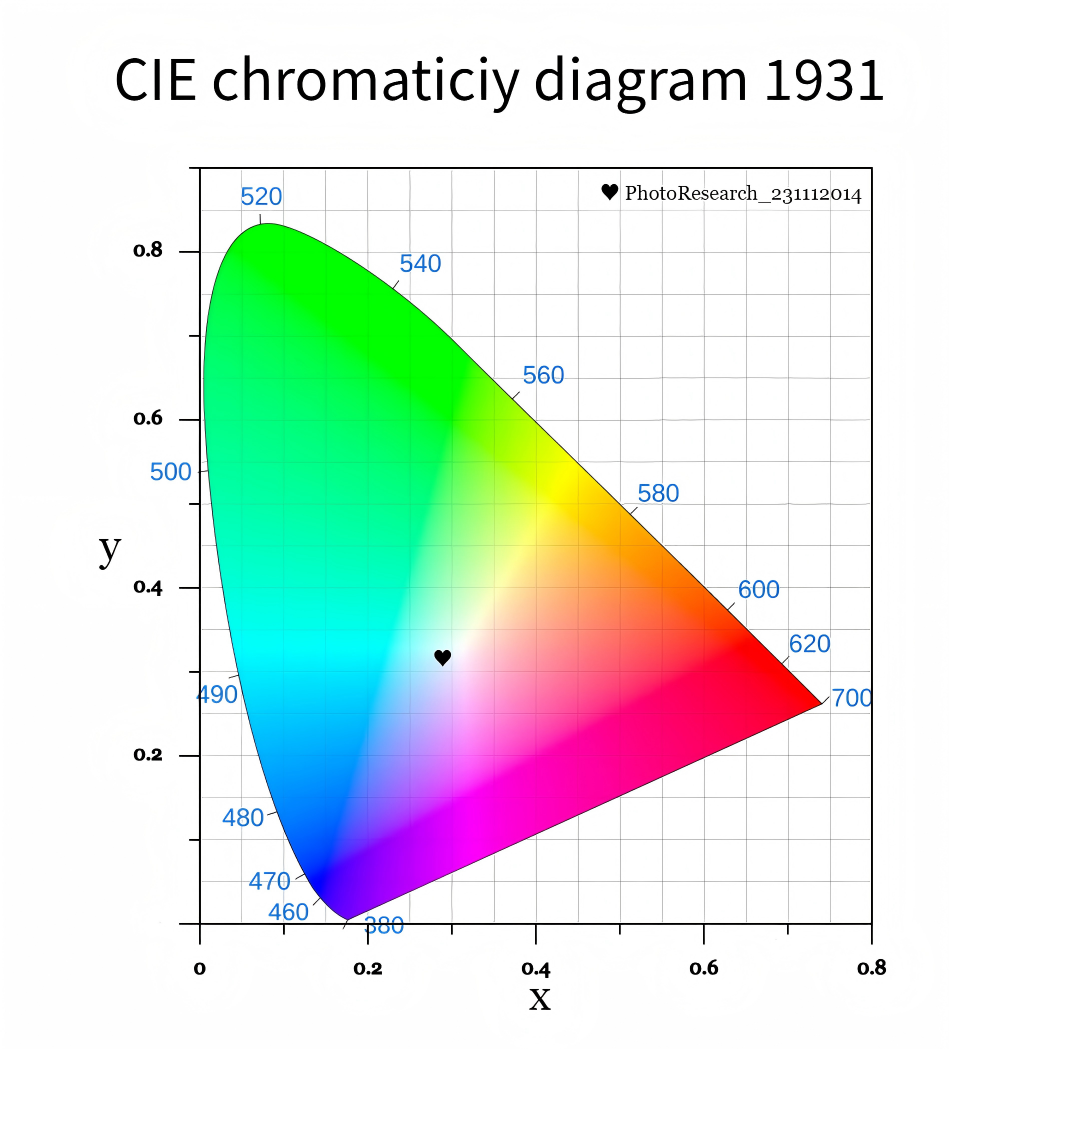
\includegraphics[width=0.6\textwidth]{CIE1931chromaticitydiagram.png}
    \caption{CIE 1931 $xy$ 色品图}
    \label{fig:cie1931}
\end{figure}

\subsection{Python 代码实现}
接续上文脚本，进行归一化计算：
\begin{lstlisting}[language=Python, caption={CIE 1931 xy 坐标计算}]
# 3. 计算 CIE 1931 xy 色品坐标
sum_XYZ = X + Y + Z
x = X / sum_XYZ
y = Y / sum_XYZ

print(f"xy 坐标: x={x:.4f}, y={y:.4f}")
\end{lstlisting}

\newpage

% ==========================================
% 第三章：CIE 1976 u'v' 色品坐标计算
% ==========================================
\section{CIE 1976 $u'v'$ 色品坐标计算}

\subsection{计算公式与分母推导}
CIE 1931 色品图存在严重的视觉不均匀性（特别是绿色区域的宽容度过大）。为解决此问题，CIE 制定了 1976 均匀色彩空间（UCS）。其坐标 $u', v'$ 可直接由 $X, Y, Z$ 推导：
\begin{align}
    u' &= \frac{4X}{X + 15Y + 3Z} \\
    v' &= \frac{9Y}{X + 15Y + 3Z}
\end{align}

为清晰展示推导过程，首先计算转换公式的分母项 $D$：
\begin{align*}
    D &= X + 15Y + 3Z \\
      &= 829.7548 + 15 \times 917.9431 + 3 \times 1175.6139 \\
      &= 829.7548 + 13769.1465 + 3526.8417 \\
      &= 18125.7430
\end{align*}

\subsection{最终计算结果与可视化}
分别计算分子并除以分母 $D$：
\begin{align*}
    u' &= \frac{4 \times 829.7548}{18125.7430} = \frac{3319.0192}{18125.7430} \approx \mathbf{0.1831} \\
    v' &= \frac{9 \times 917.9431}{18125.7430} = \frac{8261.4879}{18125.7430} \approx \mathbf{0.4558}
\end{align*}

该目标白场点坐标在均匀色品图上的位置如图 \ref{fig:cie1976} 所示。

\begin{figure}[H]
    \centering
    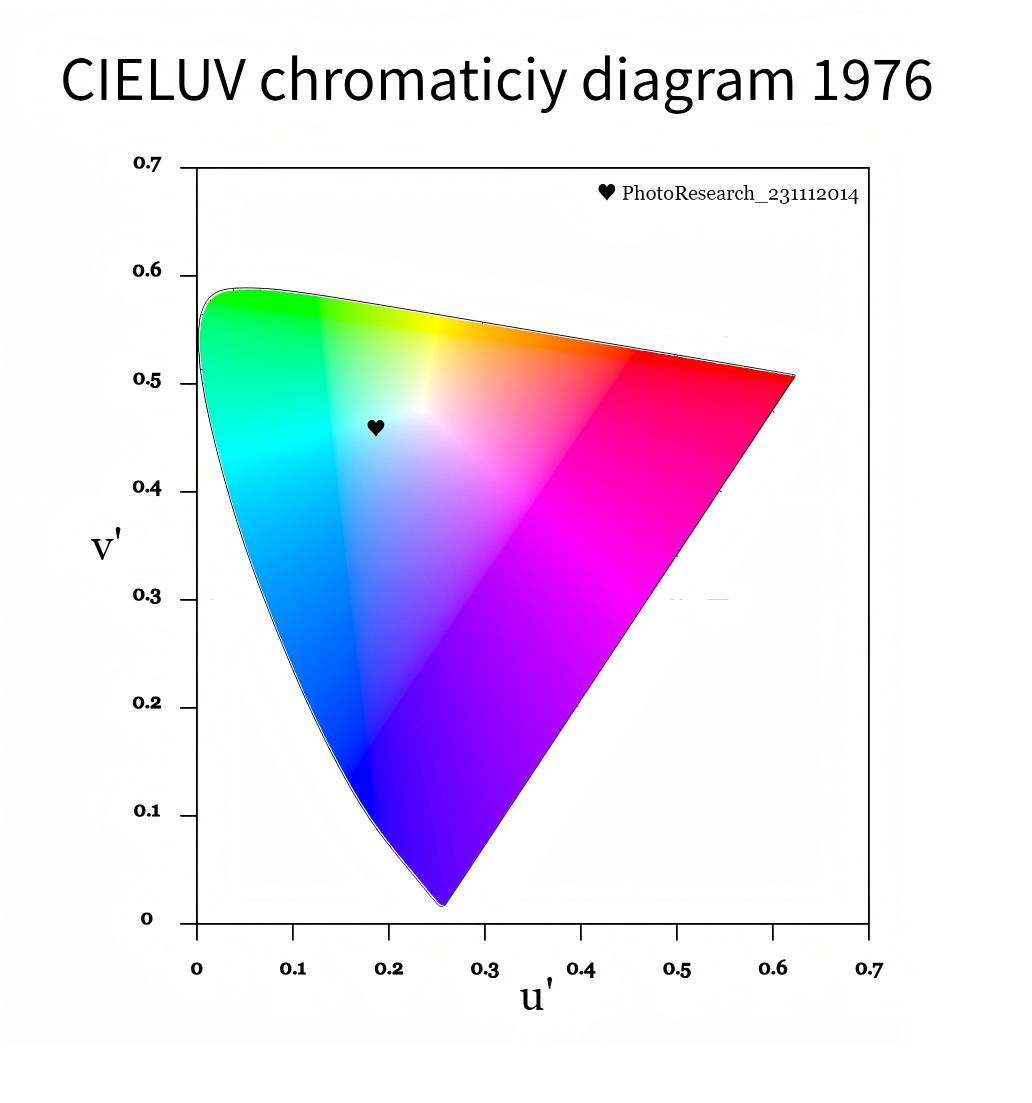
\includegraphics[width=0.6\textwidth]{CIE1976chromaticitydiagram.png}
    \caption{CIE 1976 $u'v'$ 色品图}
    \label{fig:cie1976}
\end{figure}

\subsection{Python 代码实现}
接续上文脚本，进行 UCS 坐标投影：
\begin{lstlisting}[language=Python, caption={CIE 1976 u'v' 坐标计算}]
# 4. 计算 CIE 1976 u'v' 均匀色彩空间坐标
denominator = X + 15 * Y + 3 * Z
u_prime = (4 * X) / denominator
v_prime = (9 * Y) / denominator

print(f"u'v' 坐标: u'={u_prime:.4f}, v'={v_prime:.4f}")
\end{lstlisting}

\newpage

% ==========================================
% 第四章：相关色温 (CCT) 计算
% ==========================================
\section{相关色温 (CCT) 计算}

\subsection{计算公式与中间变量逼近}
针对测得的色品坐标，本实验采用经典的 \textbf{McCamy (1992)} 三次多项式逼近算法来计算相关色温（CCT）。该算法通过建立等温线（Isotemperature lines）的近似斜率方程，实现从 $xy$ 坐标到色温的快速转换。

首先计算中间变量 $n$（代表色坐标相对于光源起点的倒数斜率）：
\begin{equation}
    n = \frac{x - x_e}{y_e - y} 
\end{equation}
式中，经验常数设定为 $x_e = 0.3320, y_e = 0.1858$。

接着利用三次多项式拟合曲线计算最终色温：
\begin{equation}
    \mathrm{CCT} = 449n^3 + 3525n^2 + 6823.3n + 5520.33
\end{equation}

\subsection{逐项展开计算结果与可视化}
代入本实验测得的坐标近似值 $x \approx 0.2838, y \approx 0.3140$，求得 $n$：
\begin{equation*}
    n = \frac{0.2838 - 0.3320}{0.1858 - 0.3140} = \frac{-0.0482}{-0.1282} \approx 0.375975
\end{equation*}

为保证多项式精度，先求出 $n$ 的高次项：
\begin{align*}
    n^2 &\approx 0.141357 \\
    n^3 &\approx 0.053147
\end{align*}

将各项分别代入公式：
\begin{align*}
    \mathrm{CCT} &\approx 449 \times 0.053147 + 3525 \times 0.141357 + 6823.3 \times 0.375975 + 5520.33 \\
        &\approx 23.863 + 498.283 + 2565.388 + 5520.33 \\
        &\approx \mathbf{8607.864 \text{ K}} \approx \mathbf{8608 \text{ K}}
\end{align*}

结合测得的坐标在黑体辐射轨迹（Planckian Locus）附近的局部放大图（如图 \ref{fig:cct} 所示，图表参考自 \href{https://www.waveformlighting.com/tech/calculate-color-temperature-cct-from-cie-1931-xy-coordinates}{Waveform Lighting}），可以看出该显示屏白场的相关色温约为 8608 K。在影视制作流程中，这一数值显著高于 D65 工业标准（6504 K），意味着如果不做进一步的硬件校准，该监视器在回放素材时会表现出明显的偏蓝冷色调。

\begin{figure}[H]
    \centering
    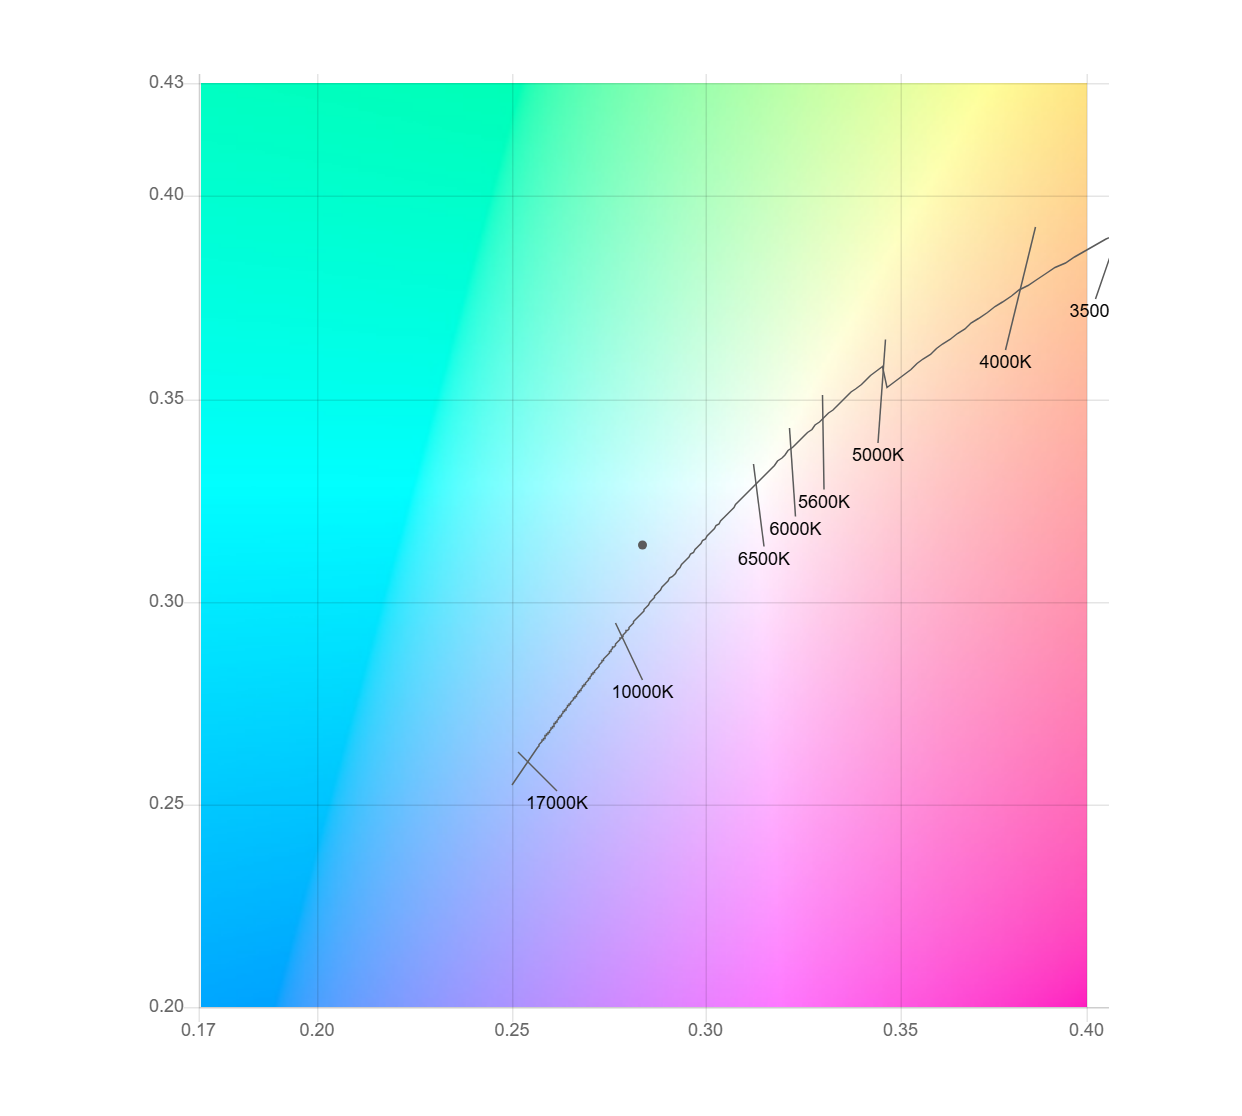
\includegraphics[width=0.8\textwidth]{cct.png}
    \caption{CCT 局部放大图与黑体辐射轨迹}
    \label{fig:cct}
\end{figure}

\subsection{扩展：其他色温算法推导与对比}
为追求更高的计算精度与严谨性，本节引入另外两种学术界与工业界常用的色温计算模型进行交叉验证。

\subsubsection{Hernández-Andrés 等人指数近似算法 (1999)}
McCamy 算法在极高色温区间的误差会逐渐增大，而 Hernández-Andrés 算法采用多项指数函数拟合，在极宽广的色温范围（至 $10^5 \text{ K}$）内依然能保持高精度。

其常数与中心点偏移量 $n$ 的定义如下：
\begin{equation}
    n = \frac{x - 0.3366}{y - 0.1735}
\end{equation}

代入本实验测得的 $x \approx 0.2838, y \approx 0.3140$：
\begin{equation*}
    n = \frac{0.2838 - 0.3366}{0.3140 - 0.1735} = \frac{-0.0528}{0.1405} \approx -0.3758
\end{equation*}

利用包含自然常数 $e$ 的公式求相关色温：
\begin{align*}
    \mathrm{CCT}_{HA} &= -949.86315 + 6253.80338 \exp\left(-\frac{n}{0.92159}\right) \\
    &\quad + 28.70599 \exp\left(-\frac{n}{0.20039}\right) + 0.00004 \exp\left(-\frac{n}{0.07125}\right) \\
    &\approx -949.86 + 6253.80(1.503) + 28.71(6.523) + 0.00004(195.27) \\
    &\approx -949.86 + 9402.34 + 187.25 + 0.01 \\
    &\approx \mathbf{8640 \text{ K}}
\end{align*}

\subsubsection{CIE 1960 UCS 最小几何距离法 (Robertson, 1968)}
此为 CIE 官方推荐的标准逻辑。通过将坐标转换至 CIE 1960 $uv$ 均匀色彩空间，寻找该点到黑体辐射轨迹（Planckian Locus）等温线的最短垂直距离。

坐标转换公式为：
\begin{align}
    u &= \frac{4x}{-2x + 12y + 3} \\
    v &= \frac{6y}{-2x + 12y + 3}
\end{align}

代入数据推导分母 $D_{1960}$ 与坐标：
\begin{align*}
    D_{1960} &= -2(0.2838) + 12(0.3140) + 3 = 6.2004 \\
    u &= \frac{1.1352}{6.2004} \approx \mathbf{0.1831} \\
    v &= \frac{1.8840}{6.2004} \approx \mathbf{0.3039}
\end{align*}

根据标准 Robertson 算法在黑体辐射数据表中进行线性插值，得出该点距黑体辐射轨迹最近的色温值约为 $\mathbf{8635 \text{ K}}$。

\subsubsection{算法结果对比与工业指导意义}
将三种算法的计算结果汇总如下：
\begin{itemize}
    \item \textbf{McCamy (1992)}: $\mathbf{8608 \text{ K}}$
    \item \textbf{CIE Robertson (1968)}: $\mathbf{8635 \text{ K}}$
    \item \textbf{Hernández-Andrés (1999)}: $\mathbf{8640 \text{ K}}$
\end{itemize}
三种算法的最大差值仅为 32K，相对误差不足 $0.4\%$，互相印证了计算的准确性。在实际的影视前期 DIT 监看与后期 DI 调色环节，无论采用哪种底层算法，该显示屏白场均被判定为严重偏冷（远超 D65 工业标准的 6504K），需重新进行 3D LUT 校准或硬件白平衡调整。

\subsection{Python 代码实现（包含所有色温算法）}
在原有代码基础上，追加 Hernández-Andrés 算法与 CIE 1960 转换的 Python 代码：
\begin{lstlisting}[language=Python, caption={多种相关色温（CCT）算法对比计算}]
import math

# 1. 计算 McCamy 相关色温 CCT
x_e = 0.3320
y_e = 0.1858

n = (x - x_e) / (y_e - y)
CCT_McCamy = 449 * (n**3) + 3525 * (n**2) + 6823.3 * n + 5520.33
print(f"McCamy 算法计算所得 CCT: {CCT_McCamy:.0f} K")

# 2. Hernandez-Andres 算法
n_ha = (x - 0.3366) / (y - 0.1735)
CCT_HA = -949.86315 + 6253.80338 * math.exp(-n_ha / 0.92159) + \
         28.70599 * math.exp(-n_ha / 0.20039) + \
         0.00004 * math.exp(-n_ha / 0.07125)
print(f"Hernandez-Andres 算法计算所得 CCT: {CCT_HA:.0f} K")

# 3. CIE 1960 UCS 坐标转换 (用于 Robertson 插值)
den_1960 = -2 * x + 12 * y + 3
u_1960 = (4 * x) / den_1960
v_1960 = (6 * y) / den_1960
print(f"CIE 1960 UCS 坐标: u={u_1960:.4f}, v={v_1960:.4f}")
# 结合标准色温表查表插值可得约 8635 K
\end{lstlisting}

\end{document}